We propose a parallel algorithm based in the construction of the
\emph{Range Min-Max Tree}, {\tt
  RMMT}. Our algorithm, called
\emph{Parallel Succinct Tree Algorithm}, {\tt PSTA}, has as input a
tree on $n$ nodes stored as a sequence of balanced parentheses, $P$, of
size $2n$.

%The {\tt RMMT} is constructed over $P$, partitioning $P$ in disjoint
%chunks of size $s$. Considering those chunks, the construction of the
%{\tt RMMT} is based in the computation of different arrays of size
%$O(\frac{N}{s})$. Such arrays are $e^{\prime}$, saving the final
%excess of each chunk, $m^{\prime}$, saving the minimum excess value of
%each chunk, $M^{\prime}$, saving the maximum excess value of each
%chunk and $n^{\prime}$, saving the number of ocurrences of the minimum
%value of each chunk. As a reminder, the excess value at position $i$
%is:
%\begin{equation}
%  \displaystyle E[i] = \sum_{k=0}^{i} \pi(P[k])
%  \label{eq:excess}
%\end{equation}

%where $\pi(``(") = 1$ and $\pi(``)") = -1$. See Figure
%\ref{fig:RangeMinMaxTree} as an example of {\tt RMMT}, with $s=3$ and
%$k=3$.

%\begin{figure}[ht]
%  \centering
%  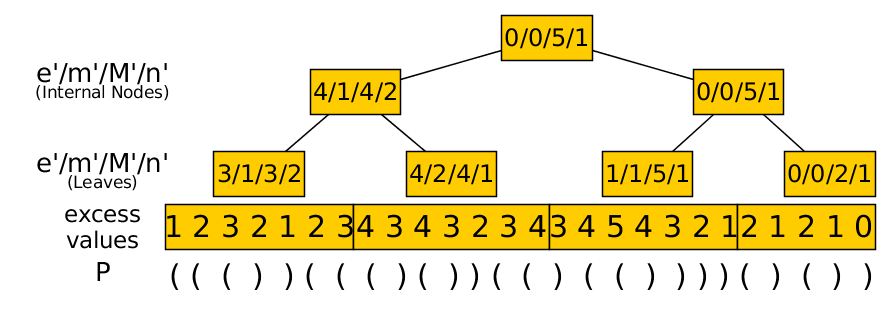
\includegraphics[scale=0.18]{./images/Range-min-max-tree.png}
%  \caption{Range min-max tree}
%  \label{fig:RangeMinMaxTree} 
%\end{figure}

The first step of {\tt PSTA} is to compute the arrays $e^{\prime}$,
$m^{\prime}$, $M^{\prime}$ and $n^{\prime}$ in parallel. Since
$e^{\prime}$ just saves the last excess value of each chunk, which is
a sum, {\tt PSTA} needs to apply a parallel prefix sum
algorithm. Computing the last element of $e^{\prime}$, at position
$\frac{2n}{s}-1$, we indirectly compute the rest of the elements of
$e^{\prime}$. We adapted the algorithm in \cite{Helman2001265} for
this context, computing $e^{\prime}$ in $O(\frac{n}{p}+\lg p)$ time, using
$p$ threads. Note that we do not need to compute more elements of
$e^{\prime}$ to the internal nodes of the {\tt RMMT}. The memory used
in construction time are bounded by $O(n\lg(n))$ bits.

To compute $m^{\prime}$, let's assume, without loss of generality,
that $p = k^{i}$, where $k$ is the arity
of the internal nodes in the {\tt RMMT} and $i > 0$. {\tt PSTA}
assigns one thread per sub-tree of size $O(\frac{n}{sp})$, at level
$i$. So, it is possible to compute the $m^{\prime}$ values in all
sub-trees, in parallel, in $O(\frac{n}{sp}k)$ time. Then, for the
rest $O(p)$ nodes in the top of the tree, we compute the corresponding
minimum values in $O(k\lg_{k} p)$ time, computing each level in $O(k)$
time, just looking the $k$ values on the previous level using one
thread per vertex. If we consider $s$ and $k$ as constants, we can compute
$m^{\prime}$ in
$O(\frac{n}{sp}k + \lg p) = O(\frac{n}{p}+\lg p)$ \Jose{$s$ and $k$ constants?}time,
using $O(n\lg(n))$ bits in construction time and in the
final array. Note that this solution makes sense considering that
$p\ll N$. Figure \ref{fig:min-max-array} illustrates the solution
explained here. We can compute $M^{\prime}$ and $n^{\prime}$ in the
same way, obtaining the same complexity.

\begin{figure}[t]
  \centering
  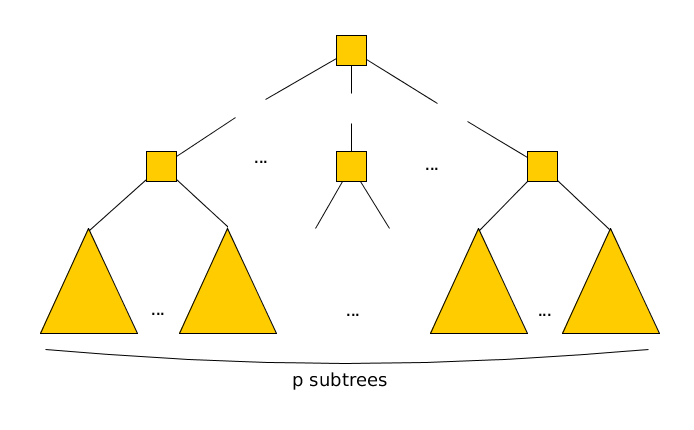
\includegraphics[scale=0.28]{./images/Min-Max-array.png}
  \caption{Computation of $m^{\prime}$ and $M^{\prime}$}
  \label{fig:min-max-array} 
\end{figure}

In addition to the arrays, the construction of the {\tt RMMT} involves
the computation of \emph{universal tables}.
%The universal tables are
%used to support \emph{fwd\_search}($\bullet$),
%\emph{bwd\_search}($\bullet$), \emph{rmqi}($\bullet$),
%\emph{RMQi}($\bullet$), \emph{degree}($\bullet$) and
%\emph{child}($\bullet$) queries.
We can divide
universal tables into two types: those that depend on the leaves of
the {\tt RMMT} and those that depend on the internal nodes. In the
first case, we can compute each universal table in parallel assigning
one processor per leaf or chunk, which allows to compute different
parts of the table at the same time. For the second kind of tables, we
can assign one processor per internal node. Such processor computes
the section corresponding to that internal node in the universal
table. In that way, since computing the universal tables sequentially
has a complexity of $O(\sqrt{2^{w}}poly(w))$ time according to
\cite{Navarro:2014:FFS:2620785.2601073}, we can compute those
universal tables in $\displaystyle O(\frac{\sqrt{2^{w}}poly(w)}{p})$,
using $p$ processors.

To reduce the space used by the {\tt RMMT}, Sadakane and Nava\-rro used
the \emph{aB-tree}. As the {\tt RMMT} and aB-tree are both complete trees, we can apply a
construction as that shown in Figure \ref{fig:min-max-array} to
construct the aB-tree. With respect to the universal tables needed in
the aB-tree, they can be computed following the same strategy
explained previously, but now with size $O(\sqrt{2^{w}})$
bits.

Finally, we can modify Theorem 4 of
\cite{Navarro:2014:FFS:2620785.2601073} as follows:

\newtheorem{theorem}{Theorem}
\begin{theorem}
  We can represent a parentheses sequence $P$ of size $2n$, computing all
  operations of Table \ref{tbl:operations}
  in $O(\lg n)$ time, with a data
  structure depending on $P$ that uses $2n+o(n)$ bits, and universal
  tables (i.e., not depending on $P$) that use $O(\sqrt{2^{w}}poly(w))$
  bits, where $w$ is the word size of the RAM model. The preprocessing
  time is $O(\frac{n}{p} + \lg p)$, using $p$
  processors, and its working space is $O(n\lg n)$ bits.
\end{theorem}
			
When we talk about a $w$-bit word RAM, we mean a model that supports
parallelism and can manipulate $w$ bits in $O(1)$. DYM meets these
criteria. Additionally, we consider that the overhead (in space and
time) imposed by the scheduling of processors is negligible. This is
reflected in the results of \cite{Blumofe:1999:SMC:324133.324234} and in the fact that the number of available processing units in current systems is generally much lower than the input $n$.
